\section{Methodology}
\label{sec:method}

\subsection{Overall Framework of the Proposed SGFNet}

The overall framework of the proposed Semantic-Guided Fusion Network (SGFNet) is illustrated in Fig. \ref{fig-frame}. The framework adopts a dual-branch architecture, where the HSI and SAR/LiDAR data are first processed separately through convolutional layers to extract preliminary spectral–spatial and structural representations. To achieve effective cross-modal interaction, the network introduces multiple stacked Semantic-Guided Fusion Modules (SGFM). Within each module, a Semantic Mixing Convolution Block (SMCB) is employed to capture high-level semantic contextual information and enhance discriminative feature learning. Meanwhile, a Frequency Modulated Fusion Block (FMFB) is designed to model complementary frequency-domain characteristics between heterogeneous modalities, enabling the network to preserve fine-grained structural details and suppress redundant or noisy information. The semantic and frequency-aware features are then adaptively aggregated through residual fusion operations, promoting more robust cross-modal feature interaction.

By progressively stacking several SGFMs, the framework performs hierarchical semantic refinement and deep multi-modal feature fusion. Finally, the fused representations are integrated through two convolutional layers for refinement to further enhance category consistency and discrimination, producing the final classification results.

\begin{figure}[!t]
  \centering
  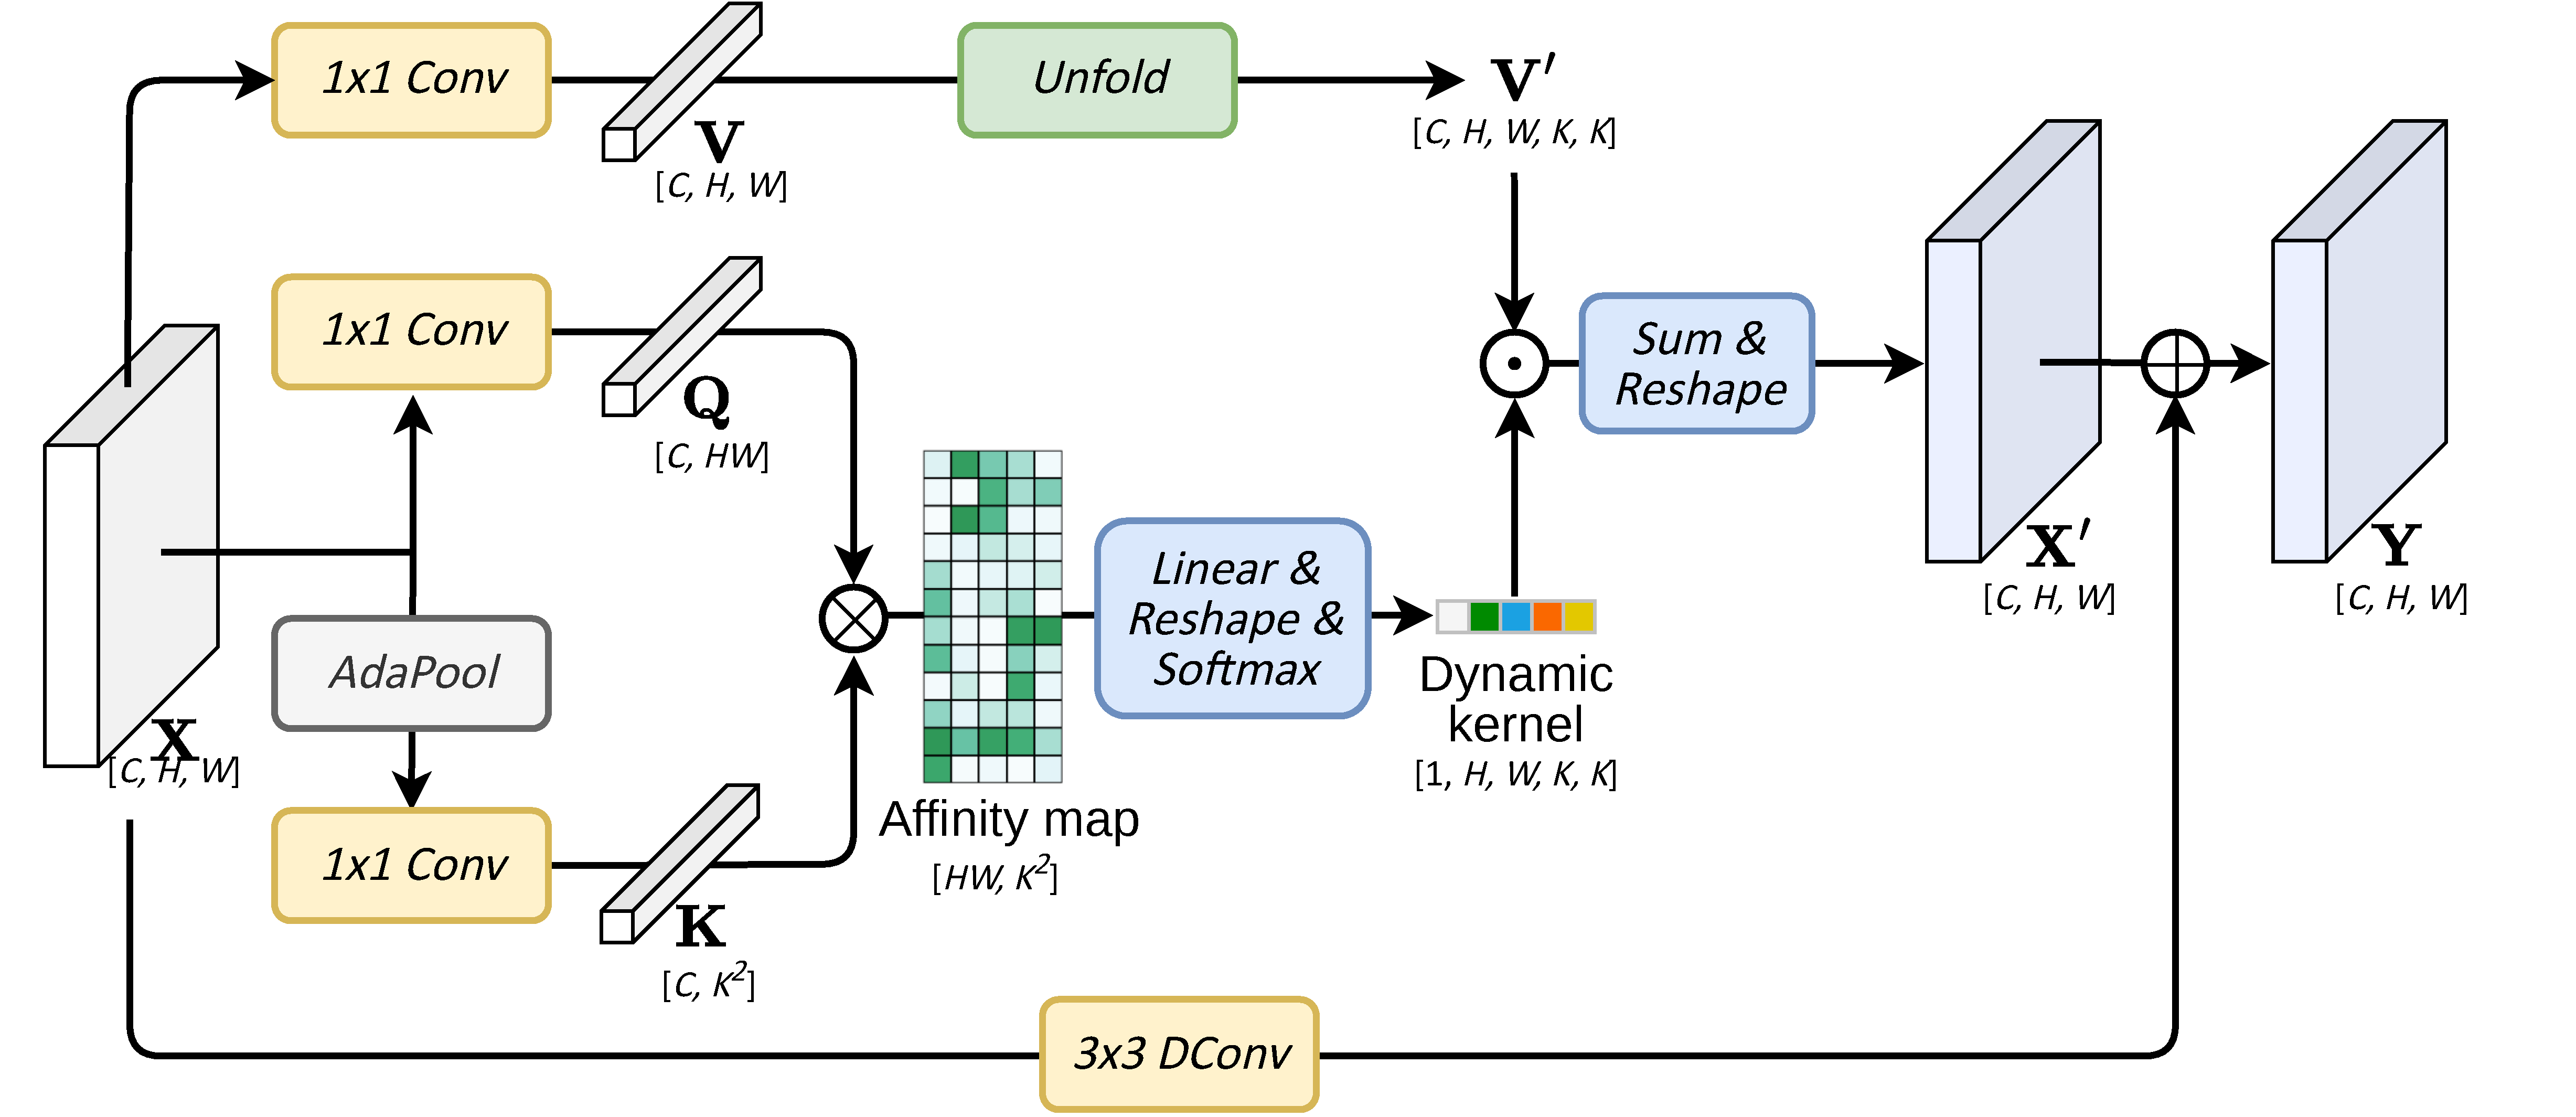
\includegraphics[width=3.2in]{figures/fig-smcb.pdf}
  \caption{Illustration of the Semantic Mixing Convolution Block (SMCB).}
  \label{fig-smcb}
\end{figure}


\subsection{Semantic Mixing Convolution Block (SMCB)}

Standard convolutions use spatially shared fixed kernels, limiting their ability to adapt to varying semantic structures and contextual relationships. To address this issue, we propose the Semantic Mixing Convolution Block (SMCB), which integrates convolution with semantic-aware dynamic filtering. Instead of fixed kernels, SMCB dynamically generates spatially adaptive kernels based on semantic affinities between query and key features. The resulting dynamic kernels guide local feature aggregation, enabling the network to emphasize semantically relevant contextual information adaptively. Details of the SMCB are shown in Fig. \ref{fig-smcb}. Given an input feature $\mathbf{X}\in\mathbb{R}^{C\times H\times W}$, it is projected by a $1\times1$ convolution to obtain the value and query features as: 
\begin{equation}
\mathbf{V}=f_v(\mathbf{X}), ~~~ \mathbf{Q}=f_q(\mathbf{X}),
\end{equation}
where $f_v$ and $f_q$ denote the convolution layer. Meanwhile, $\mathbf{X}$ is passed through an adaptive pooling layer to extract compact contextual information as:
\begin{equation}
  \mathbf{K} = f_k(\mathrm{AdaPool}(\mathbf{X})),
\end{equation}
where $f_k$ denotes the convolution layer. We obtain $\mathbf{Q}\in\mathbb{R}^{C\times HW}$ and $\mathbf{K}\in\mathbb{R}^{C\times K^2}$ via reshaping. Here $K$ denotes the dynamic kernel size. The query and key features are multiplied to obtain an affinity map:
\begin{equation}
\mathbf{A}=\mathbf{Q}^{T}\mathbf{K}.
\end{equation}

This affinity map measures the relationship between each spatial position and the $K^2$ sampling locations in a local window. It is then processed by a linear layer, reshaped, and normalized by $\mathrm{Softmax}$ to generate the dynamic convolution kernel:
\begin{equation}
\mathbf{D}=\mathrm{Softmax}(\mathrm{Reshape}(\mathrm{Linear}(\mathbf{A}))).
\end{equation}

In parallel, the value feature $\mathbf{V}$ is unfolded into local patches:
\begin{equation}
\mathbf{V}'=\operatorname{Unfold}(\mathbf{V}).
\end{equation}

The dynamic kernel $\mathbf{D}$ is then applied to the unfolded value feature. In each channel of $\mathbf{V'}$, for every spatial position $(h,w)$, the output feature is computed by weighted summation over its local $K\times K$ neighborhood as.
\begin{equation}
  \mathbf{X}'=\sum_{i=1}^{K}\sum_{j=1}^{K} \mathbf{D}_{h,w,i,j}\cdot \mathbf{V}'_{h,w,i,j}.
\end{equation}

Besides the dynamic context branch, the framework also includes a local feature enhancement branch. The original input $\mathbf{X}$ is processed by a $3\times3$ depth-wise convolution to compute $\mathbf{X}_d$. Finally, the dynamically aggregated feature $\mathbf{X}'$ is combined with the local depth-wise convolution feature through residual addition to produce the final output:
\begin{equation}
  \mathbf{Y}=\mathbf{X}'+\mathbf{X}_d.
\end{equation}

The SMCB achieves a more flexible and semantically aware feature extraction mechanism. It is particularly suitable for understanding the complex structures of remote sensing data, where both local structural details and semantic contextual dependencies are critical.


\subsection{Frequency Modulated Fusion Block}

\begin{figure}[!t]
  \centering
  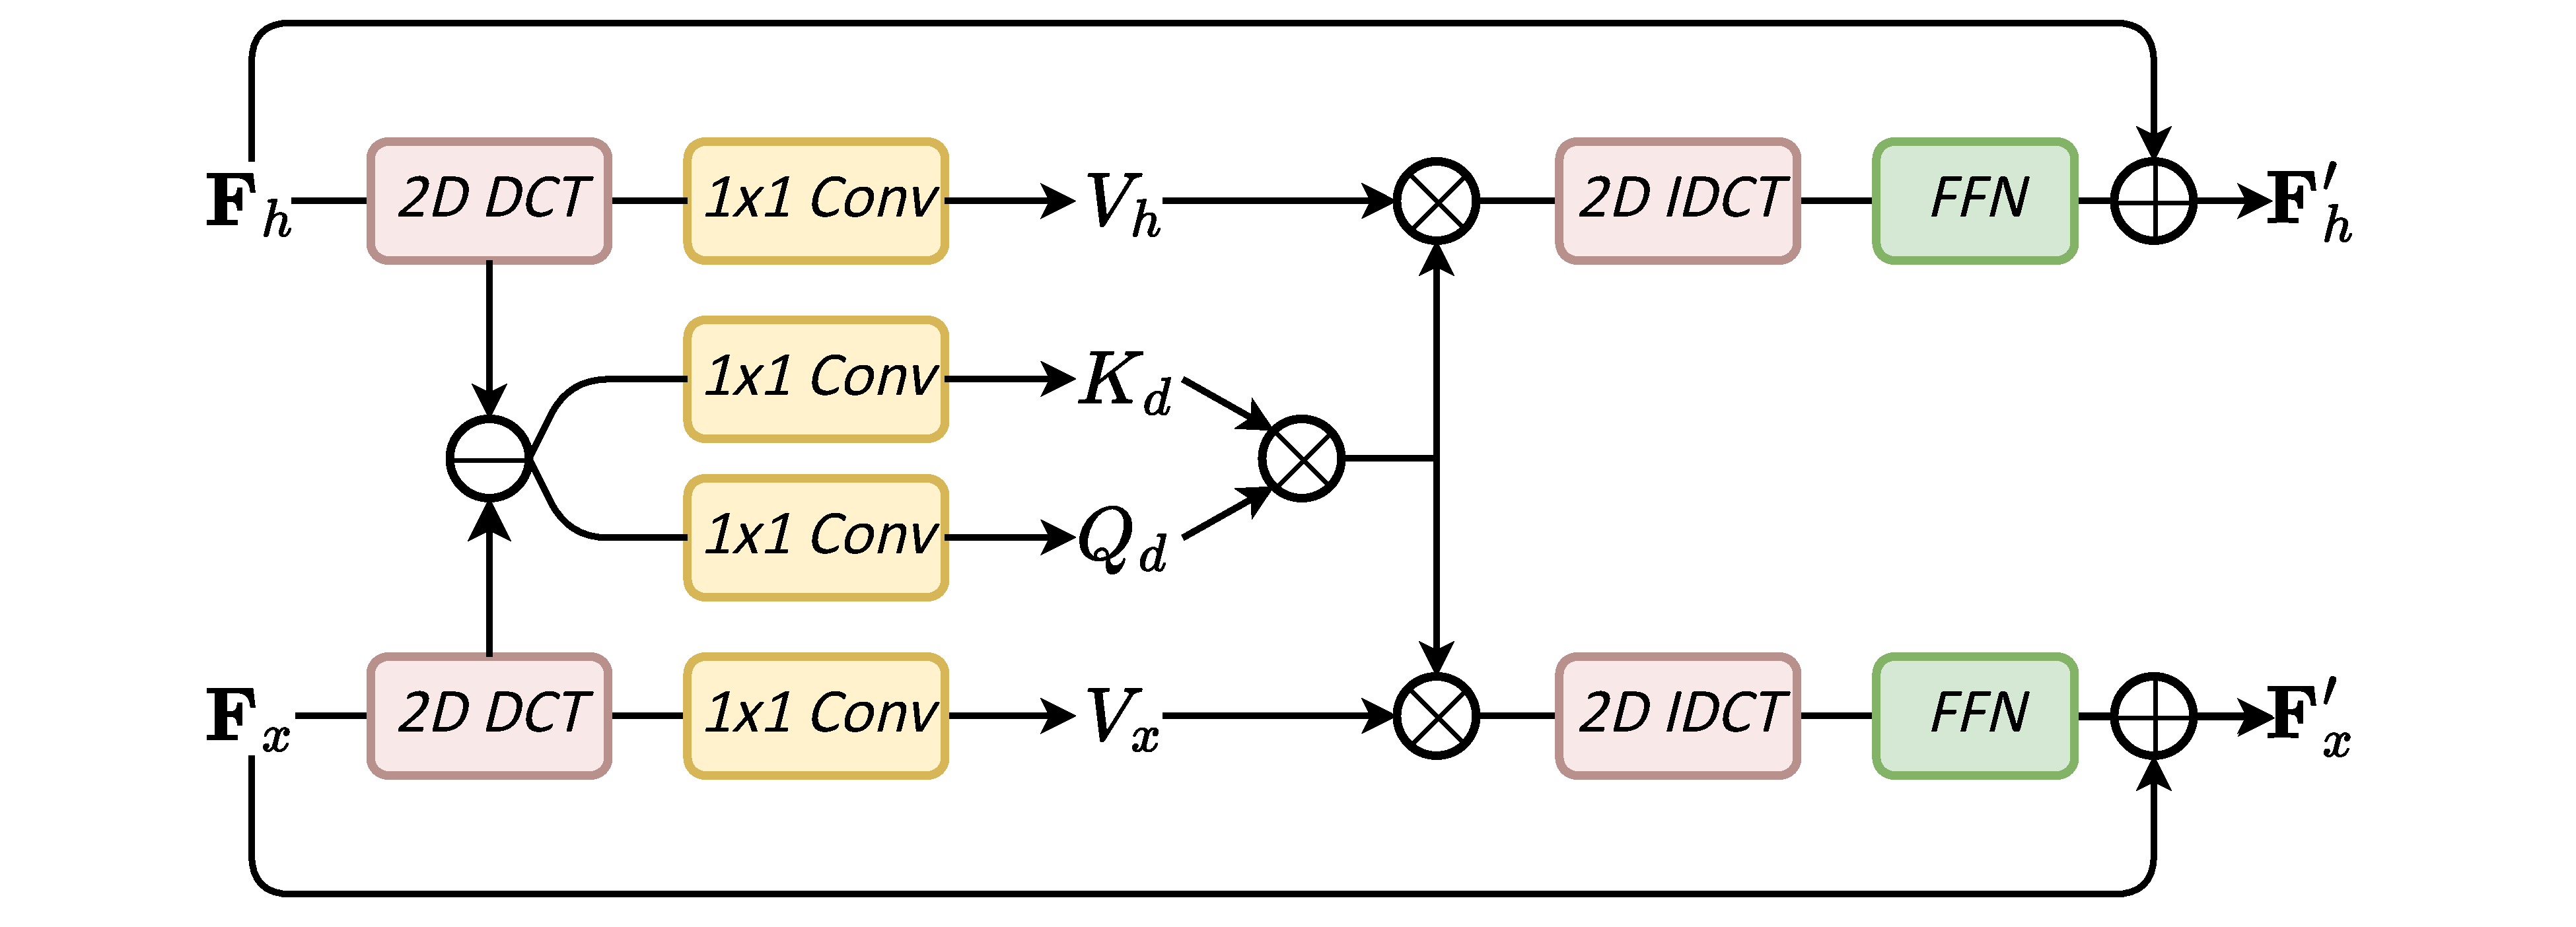
\includegraphics[width=3in]{figures/fig-fmfb.pdf}
  \caption{Illustration of the Frequency Modulated Fusion Block (FMFB).}
  \label{fig-fmfb}
\end{figure}

Multi-source data are usually collected by different sensors with varying imaging geometries and acquisition times, which often results in slight spatial misalignment between modalities. Local object regions may exhibit small positional deviations and structural inconsistencies. Such slight misalignment may weaken the effectiveness of cross-modal feature fusion. To this end, we propose the Frequency Modulated Fusion Block (FMFB), which performs adaptive cross-modal fusion in the frequency domain to enhance feature consistency.

Details of FMFB are illustrated in Fig. \ref{fig-fmfb}. It takes the feature representations $\mathbf{F}_h$ from the HSI branch and $\mathbf{F}_x$ from the SAR/LiDAR branch as inputs. It first applies 2D Discrete Cosine Transform (DCT) to project both features into the frequency domain:
\begin{equation}
\hat{\mathbf{F}}_h=\mathrm{DCT}(\mathbf{F}_h),
\quad
\hat{\mathbf{F}}_x=\mathrm{DCT}(\mathbf{F}_x).
\end{equation}

We then compute the element-wise difference in the frequency domain:
\begin{equation}
\hat{\mathbf{F}}_d=\hat{\mathbf{F}}_h-\hat{\mathbf{F}}_x.  
\end{equation}

Based on this joint representation, two $1\times1$ convolution layers generate the query and key features as $\mathbf{Q}_d=f_q(\hat{\mathbf{F}}_d)$, $\mathbf{K}_d=f_k(\hat{\mathbf{F}}_d)$. 

Meanwhile, the two DCT-transformed inputs are separately projected into value features:
\begin{equation}
\mathbf{V}_h=f_v^h(\hat{\mathbf{F}}_h),
\quad
\mathbf{V}_x=f_v^x(\hat{\mathbf{F}}_x).
\end{equation}

Next, attention is computed as follows:
\begin{equation}
 \mathbf{F}^{attn}_{h} = \mathrm{Softmax}\left(
 \frac{Q_d K_d}{\sqrt{d_k}}V_h
 \right),
\end{equation}
\begin{equation}
 \mathbf{F}^{attn}_{x} = \mathrm{Softmax}\left(
 \frac{Q_d K_d}{\sqrt{d_k}}V_x
 \right),
\end{equation}

After that, the modulated frequency-domain features are transformed back into the spatial domain through 2D inverse DCT:
\begin{equation}
\hat{\mathbf{F}}'_h=\operatorname{IDCT}(\mathbf{F}^{attn}_h),
\quad
\hat{\mathbf{F}}'_x=\operatorname{IDCT}(\mathbf{F}^{attn}_x).
\end{equation}

The reconstructed feature is further refined by the Feed-Forward Network (FFN) and residual connections:
\begin{equation}
\mathbf{F}'_h=\operatorname{FFN}(\hat{\mathbf{F}}'_h) + \mathbf{F}_h,
\quad
\mathbf{F}'_x=\operatorname{FFN}(\hat{\mathbf{F}}'_x) + \mathbf{F}_x.
\end{equation}
